\chapter{ Аналитический раздел}
\label{cha:analysis}

Lorem ipsum dolor sit amet, consectetur adipiscing elit. Integer a mauris consequat, sagittis odio ut, tempor lacus. Donec rhoncus tincidunt ligula, vel egestas turpis vehicula interdum. Phasellus sit amet dignissim metus, quis rutrum metus. Nullam euismod dictum rhoncus. Vivamus bibendum gravida lacus, iaculis consectetur nunc suscipit ac. Aliquam erat volutpat. Nulla laoreet, elit vel lacinia egestas, metus erat sagittis orci, quis vulputate urna tellus ut felis. Morbi sit amet elit auctor, ultrices dui eu, elementum nisi.



\section{Теория цвета}
Цвет можно определить как восприятие глазом и мозгом человек волн электромагнитного излучения оптического диапазона, которые преобразуются в цветовые ощущения. На возникновение цветового ощущения человека влияют зрительный опыт и память, физиологические и психологические особенности.

\subsection{Трёхкомпонентная теория цветовосприятия}
% формулки
Трёхкомпонентная теория цветовосприятия — теория, объясняющая цветовое зрение человека, основанное на восприятие трех основных компонентов цвета. В дальнейшем из научных опытов было обнаружено, что в сетчатке глаза человека существуют три вида колбочек, максимумы чувствительности которых приходятся на красный, зелёный и синий участки спектра. \cite{bib1}  Трёхсоставную теорию цветового зрения впервые высказал в 1756 году М. В. Ломоносов \cite{bib2}. Сто лет спустя её развили учёные Г. Гельмгольц, Т. Юнг и Д.К.Максвелл \cite{bib3}. Параллельно существовала оппонентная теория цвета Эвальда Геринга, которая предполагала, что в мозг поступает информацию о разнице яркости — о разнице яркости белого $Y_{max}$  и чёрного $ Y_{min}$, о разнице зелёного $G$ и красного $R$ цветов, о разнице синего$B$ и жёлтого цветов, где жёлтый цвет есть сумма красного и зелёного цветов. Её развили Дэвид Хьюбел  и Торстен Визел.  \cite{bib4}. Они получили Нобелевскую премию 1981 года за своё открытие. 
% объединить в систему 
\begin{equation}
 K_{BW} = Y_{max} - Y_{min} 
 \end{equation}
 \begin{equation}
 K_{RG}   = G - B
\end{equation}
 \begin{equation}
K_{BRG} = B - R - G, 
\end{equation}
 где $ K_{BW} $, $K_{RG}$, $K_{BRG} $ - функции коэффициентов баланса белого для любого освещения.

Эти две теории не полностью согласованы друг с другом. Но несмотря на это, до сих пор предполагают, что на уровне сетчатки действует трёхкомпонентная теория, однако информация обрабатывается и в мозг поступают данные, уже согласующиеся с оппонентной теорией. На теории о трёх составляющих цвета и строится большинство цветовых моделей. 

\subsection {Цветовые пространства и модели}
Цветовая модель -- это способ представления цвета в виде кортежа некоторых его независимых между собой характеристик. Как правило, это три составляющие его компоненты, например красный, зелёный и синий или тон, насыщенность и яркость. Цветовое пространство же -- представление цветового множества с помощью такого координатного пространства, что каждая ось преставляет возможные значения одной из компонент кортежа из цветовой модели. Необходимо четко различать цветовые модели и цветовые координатные системы: в первом случае речь идет о способе воспроизведения цветовых ощущений, а во втором — об измерении этих ощущений.

\subsubsection{CIE RGB}
Цветовая модель $RGB$ -- это аддитивная цветовая модель, в которой красный, зеленый и синий свет суммируются различными способами для воспроизведения широкого спектра цветов. Название модели происходит от инициалов трех аддитивных первичных цветов, красного $R$ , зеленого $G$ и синего $B$.
С помощью этой модели цвет можно представить в виде триплета чисел от 0 до определенного максимального значения, соответственно представляющих долю основных красного, зеленого и синего цветов. Если все компоненты равны нулю, результатом будет черный цвет; если все находятся на максимуме, результат - самый яркий представляемый белый.
Эти диапазоны можно количественно определить несколькими способами:
\begin{enumerate}
	\item От 0 до 1, с любым дробным значением между ними. Это представление используется в теоретических анализах и в системах, которые используют представления с плавающей точкой.
	\item Каждое значение цветового компонента также может быть записано в процентах от 0\% до 100\%.
	\item В компьютерах значения компонентов часто хранятся как целые числа в диапазоне от 0 до 255, диапазон, который может предложить один 8-разрядный байт. Они часто представлены как десятичные или шестнадцатеричные числа.
	\item Высококачественное цифровое графическое оборудование часто может иметь дело с большими целыми диапазонами для каждого основного цвета, например 0..1023 (10 бит), 0..65535 (16 бит) или даже больше, путем расширения 24-бит ( три 8-битных значения) до 32-разрядных , 48-битных или 64-битных единиц (более или менее независимых от размера слова конкретного компьютера )
\end{enumerate}	

\begin{figure}[ht!]
	\centering{ 
		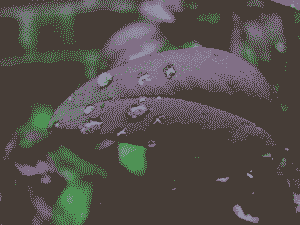
\includegraphics[width=0.4\textwidth]{img/2_bit.png}
		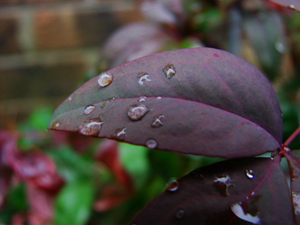
\includegraphics[width=0.4\textwidth]{img/32_bit.png}
		\caption{Cравнение изображений с глубиной цвета 2 бита (слева) и 32 бита (справа)}}
\end{figure}

Количество бит (объём памяти), используемое для хранения и представления цвета при кодировании одного пикселя называют глубиной цвета. 

В начале прошлого века Международная Комиссия по освещению (CIE —
Communication Internationale de l`Eclairage) предприняла попытку  измерить и систематизировать цветовые ощущения человека, вызываемые спектрально-чистыми
цветами, расположенными на всем протяжении видимого спектра: от фиолетового до
красного. Результатом этого эксперимента и стала модель RGB. 

\begin{figure}[ht!]
	\centering{ 
		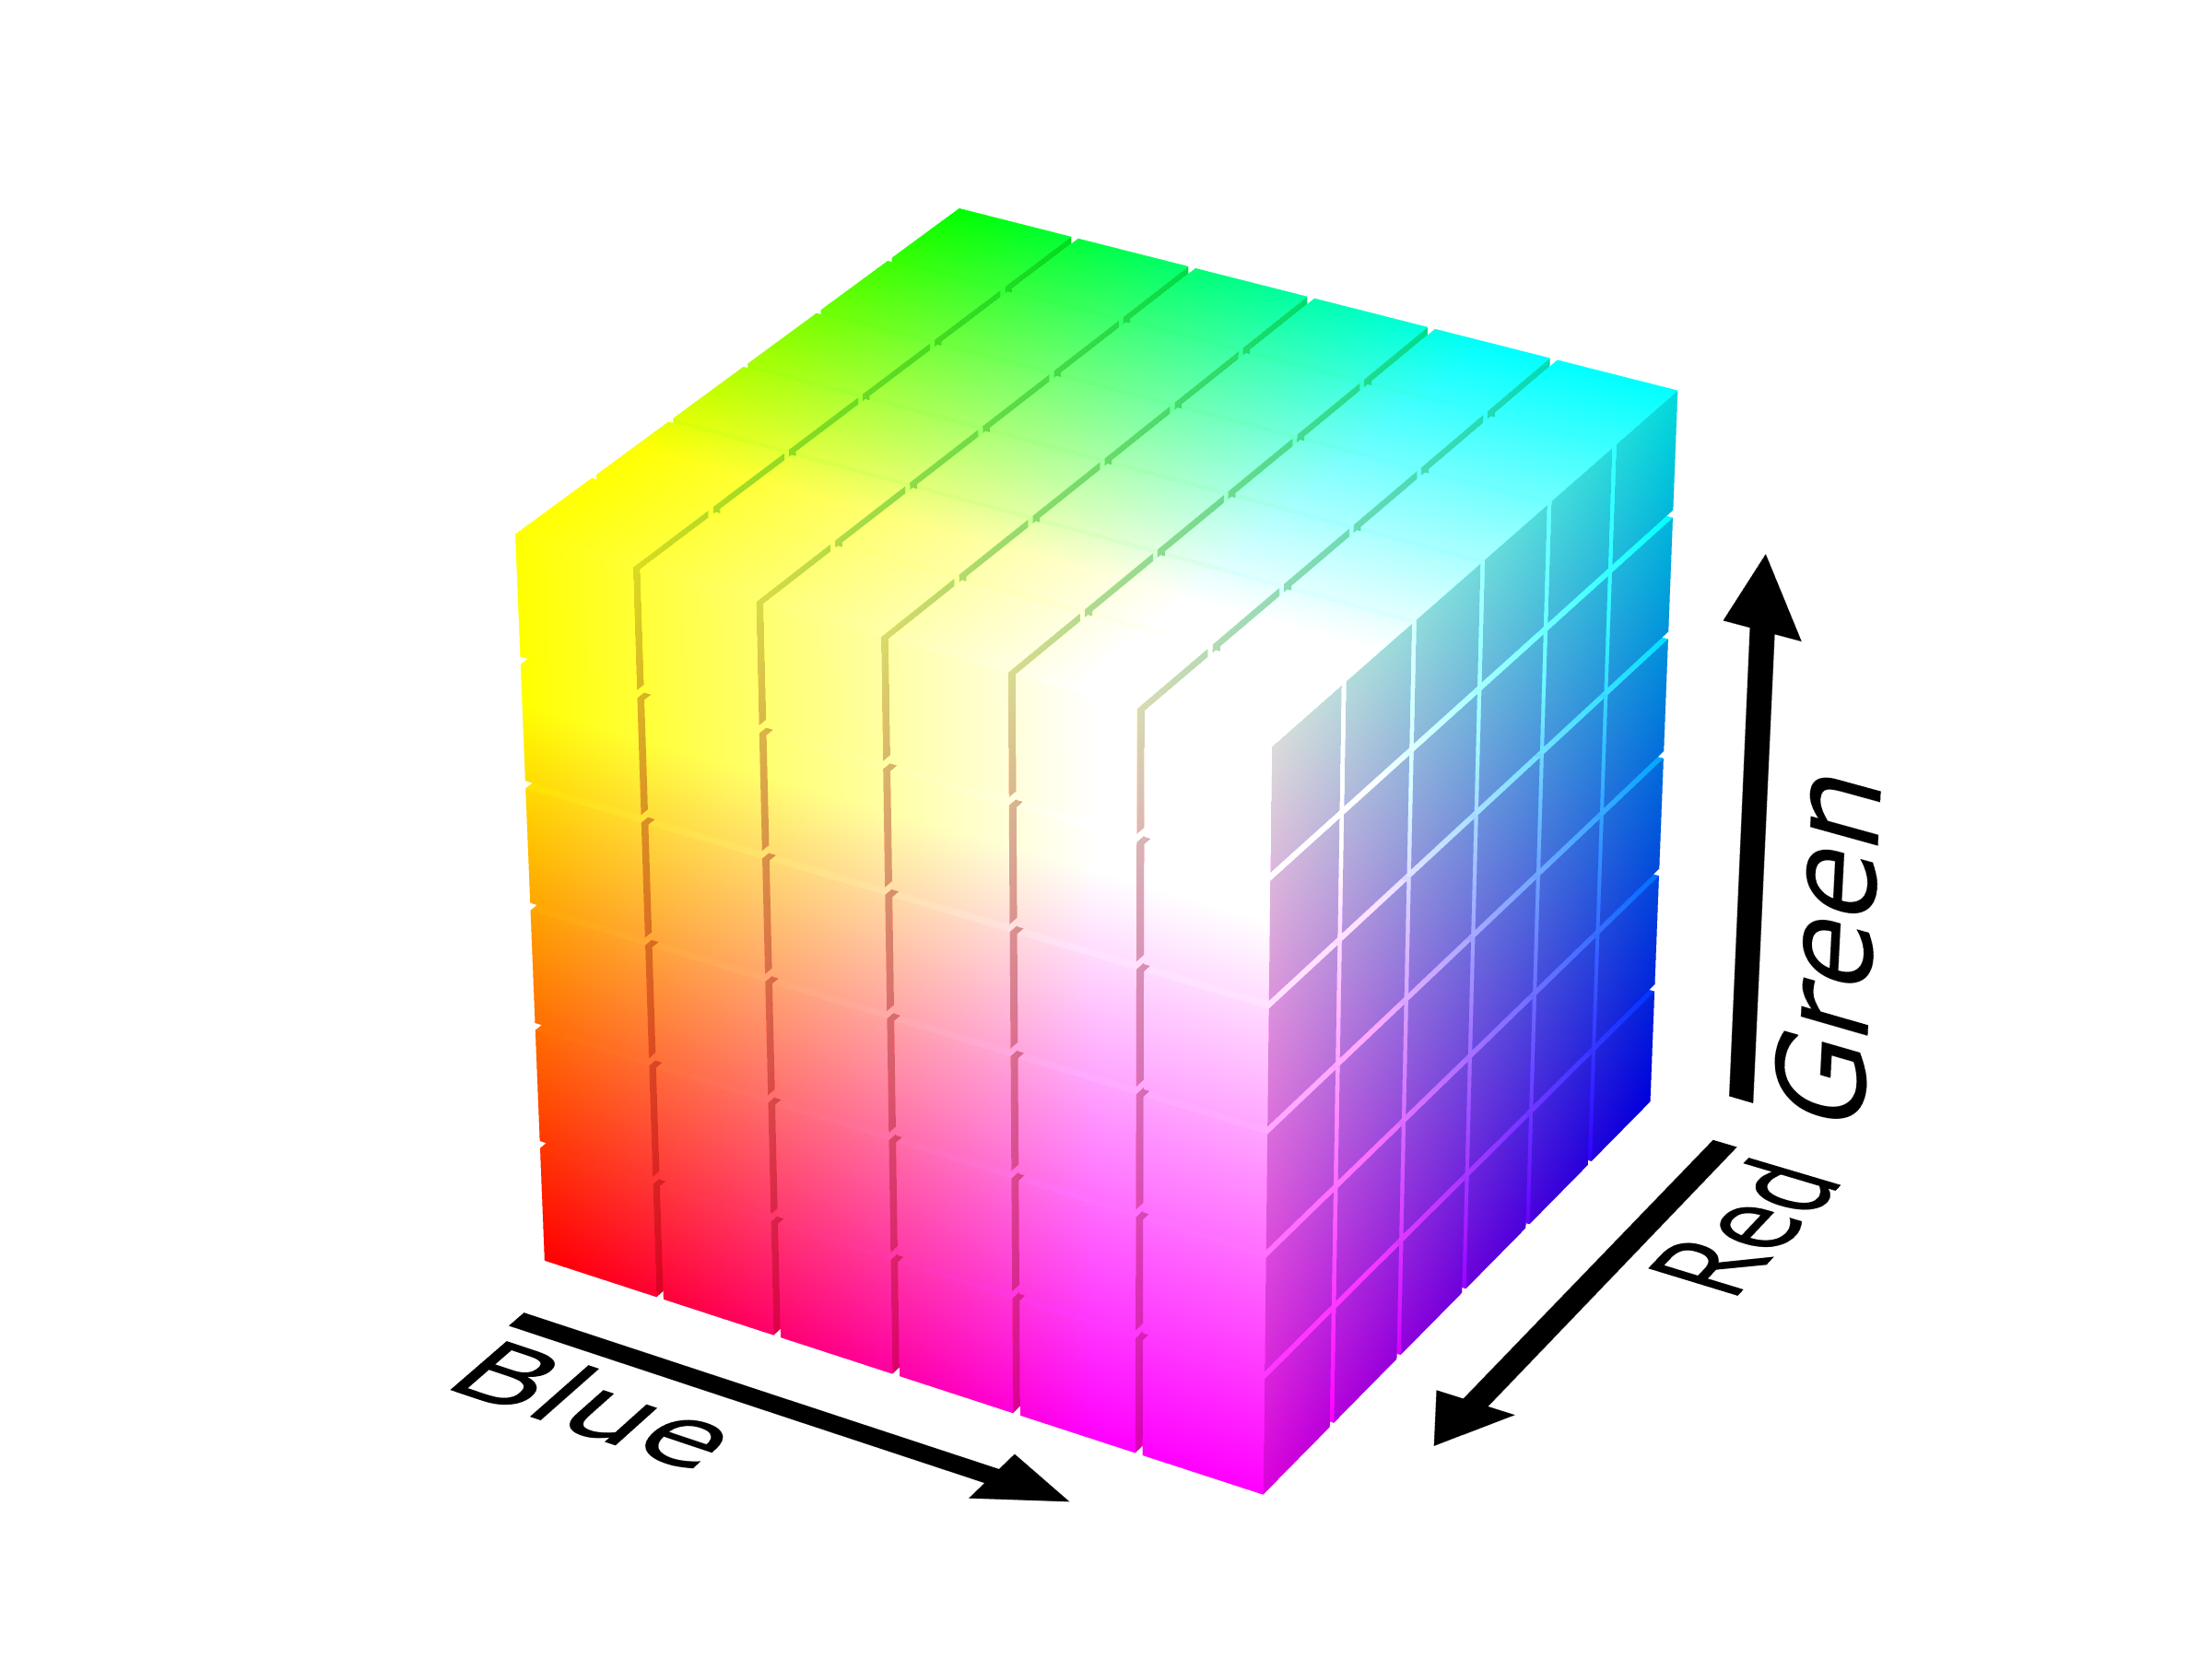
\includegraphics[width=0.4\textwidth]{img/img1.png}
		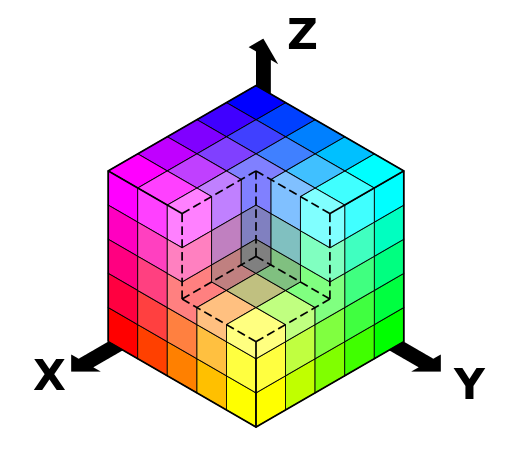
\includegraphics[width=0.4\textwidth]{img/img2.png}
		\caption{Представление цветового куба в пространстве  $RGB$ }}
\end{figure}

В эксперименте CIE существенную часть чистых спектральных цветов
уравнять не удалось (исследователи были вынуждены прибегнуть к сознательному
"загрязнению"  чистых цветов основными цветами), в результате чего в цветовой
координатной системе CIE RGB некоторые цвета имеют отрицательные координаты.
Последнее создает большие неудобства при математических расчетах. Поэтому, вскоре после возникновения CIE RGB, была предложена другая цветовая координатная система, полученная принудительным математическим пересчетом из исходной CIE RGB \cite{bib5}. 

\subsubsection{CIE 1931 XYZ}
Эта модель получила название CIE XYZ  (по трем координатным осям — XYZ). Основное ее отличие от CIE RGB - отсутствие отрицательных координат, что упрощает расчеты. Однако, как видно из вышенаписанного, сегодня модель RGB и ее производные также приведена к неотрицательным координатам.
Цветовое пространство CIE XYZ охватывает все цветовые ощущения, которые может испытать среднестатистический человек, поэтому оно является инвариантным цветовым представлением. Чтобы избежать негативных RGB значения были сформулированы «мнимые» основные цвета. Мнимые цвета не соответствуют ни одному спектральному распределению длин волн, поэтому не имеют физического смысла.  Три новых основных цвета выражались в координатах цветового пространства RGB следующим образом:

%Найти доказательство 
\begin{equation}
\overrightarrow{x} =  \begin{bmatrix} 0.41847 \\ -0.09169 \\ -0.0009209 \end{bmatrix}
\overrightarrow{y} =  \begin{bmatrix} -0.15866 \\ 0.25243 \\ -0.0025498 \end{bmatrix}
\overrightarrow{z} =  \begin{bmatrix} -0.082835 \\ 0.015708  \\ 0.17860 \end{bmatrix}
\end{equation}

Чтобы упростить визуализацию итогового цветового пространства, цвет разделяют на две части: яркость и цветность. Цветовое пространство CIE XYZ было преднамеренно спроектировано так, что параметр Y является мерой яркости цвета, известной как яркость CIE. 

\begin{figure}[ht!]
	\centering{ 
		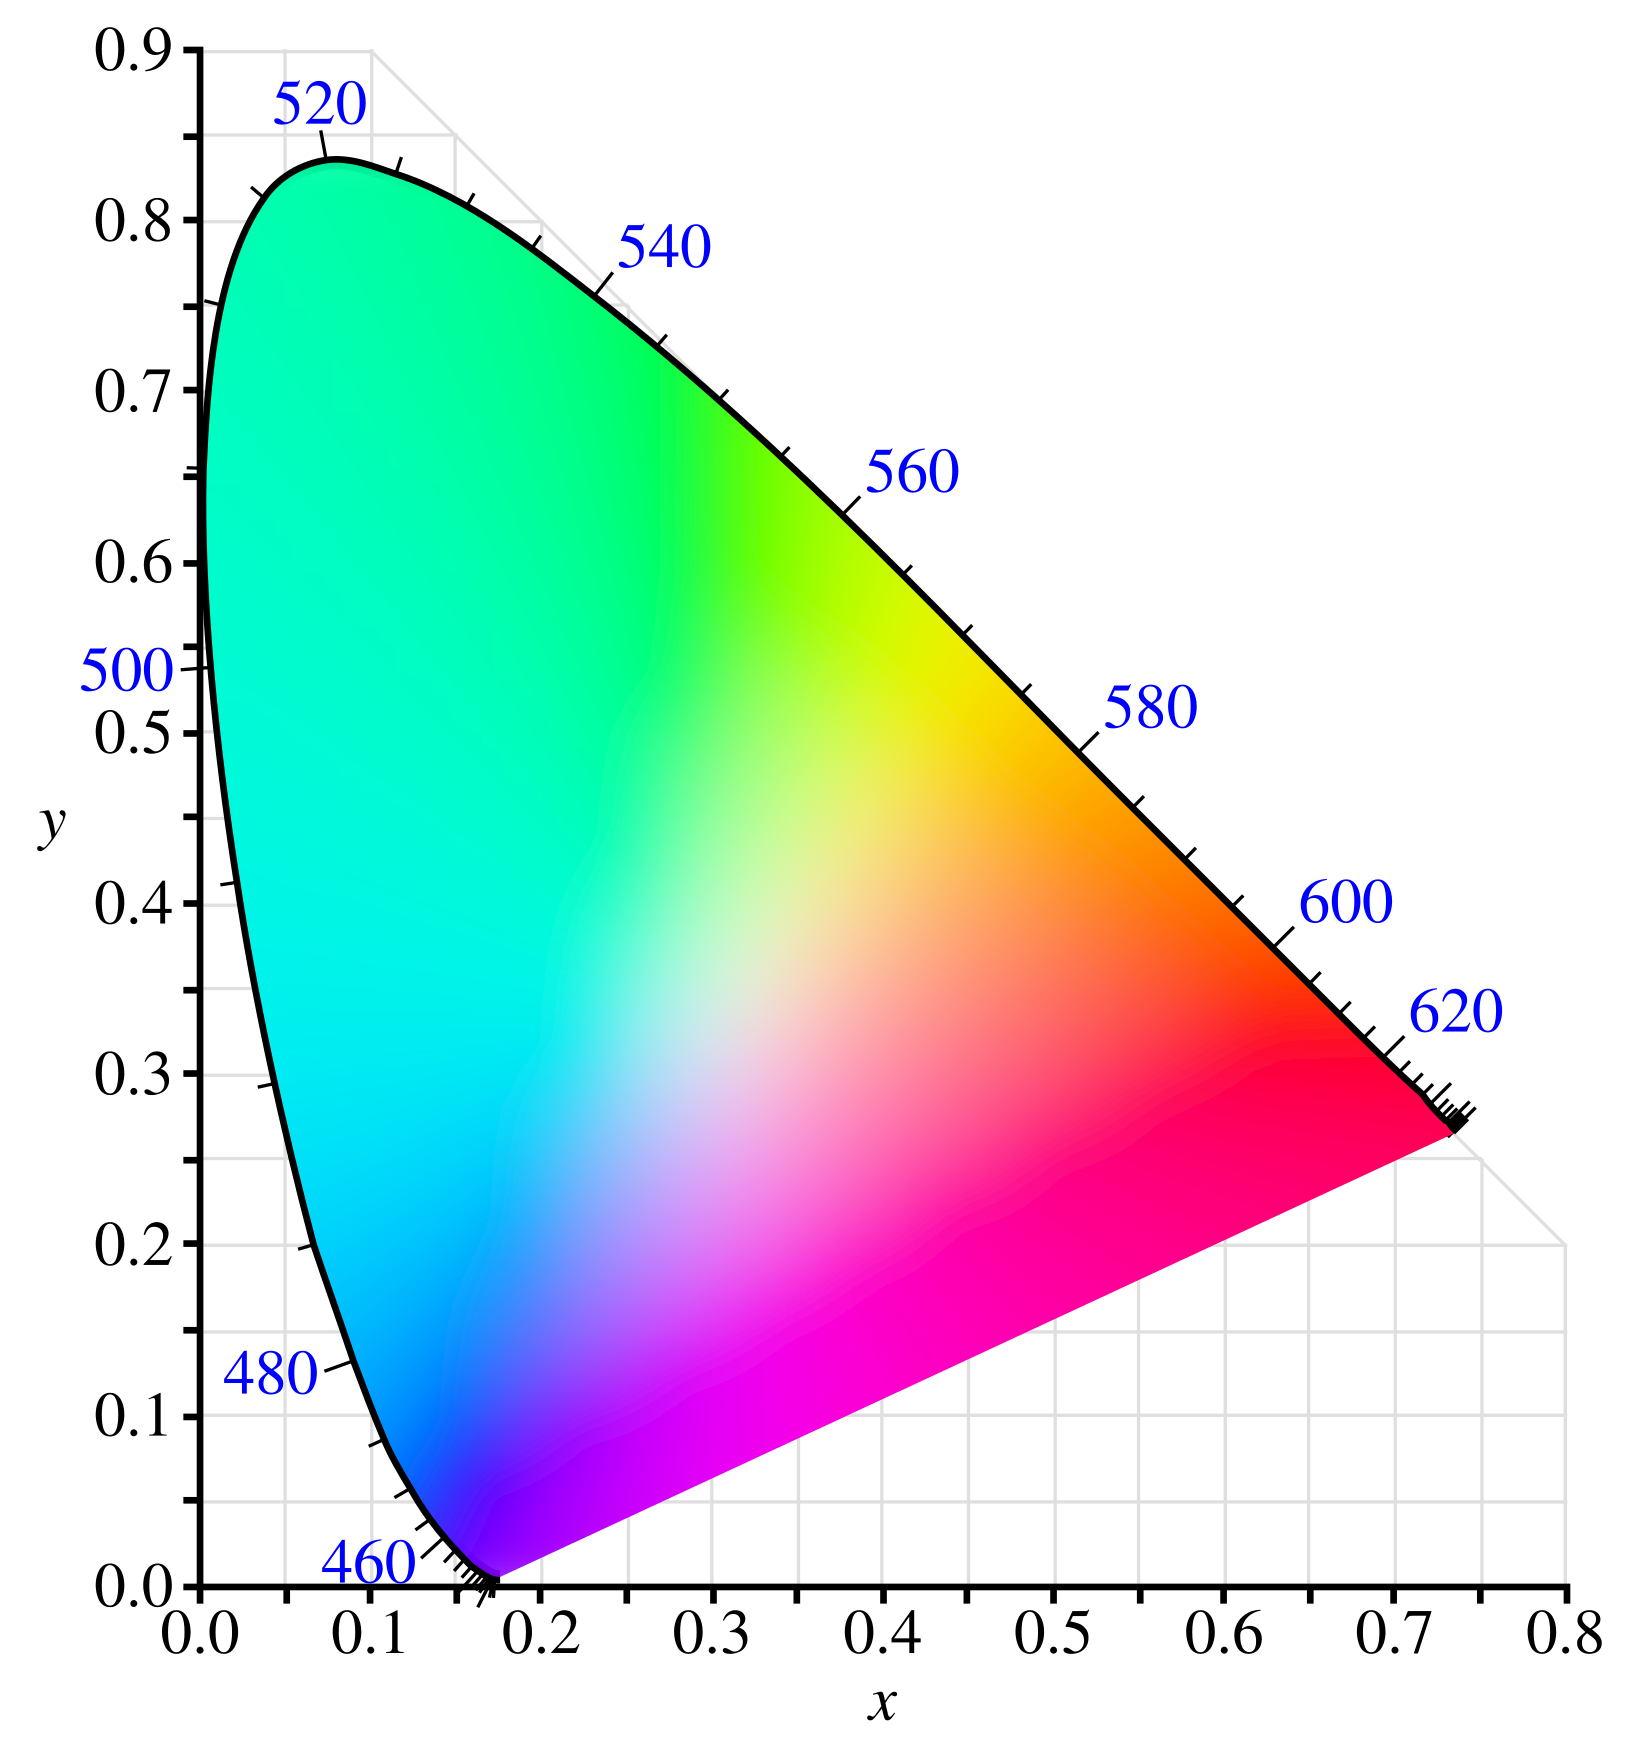
\includegraphics[width=0.4\textwidth]{img/img3.png}
		\caption{Диаграмма цветности цветного пространства CIE 1931. Прямой край в нижней части гаммы называется линией пурпурных.}}
\end{figure}

Можно получить новое цветовое пространство  CIE  xyY, где цветность цвета определяется двумя производными параметрами x и y , причем два из трех нормированных значений являются функциями всех трех значений тристимула X , Y и Z :


\begin{equation}
x = \frac{X}{X+Y+Z} 
\end{equation} 
\begin{equation}
y = \frac{Y}{X+Y+Z} 
\end{equation}
\begin{equation}
z = \frac{Z}{X+Y+Z} = 1 - x - y 
\end{equation}

Также можно вычеслить и обратные преобразования к (1.5),(1.6),(1.7):
\begin{equation}
X = \frac{Y}{y} x 
\end{equation} 

\begin{equation}
Z = \frac{Y}{y}(1 - x - y)
\end{equation} 

Диаграмма цветности иллюстрирует ряд интересных свойств цветового пространства CIE XYZ:
\begin{enumerate}
	\item Диаграмма отображает все цветности, видимые среднестатистическому человеку, и ее называют  гаммой человеческого зрения. Изогнутый край гаммы называется спектральным локусом и соответствует монохроматическому свету (каждая точка представляет собой чистый оттенок одной длины волны) с длиной волны, указанной в нанометрах (см. рисунок 1.3). Прямой край в нижней части гаммы называется линией пурпурных . Эти цвета, хотя они находятся на границе гаммы, не имеют аналогов в монохроматическом свете. Менее насыщенные цвета появляются внутри фигуры с белым в центре. 
	\item Видно, что все видимые цветности соответствуют неотрицательным значениям x , y и z (и, следовательно, неотрицательным значениям X , Y и Z ).
	\item Если выбирать любые две точки цвета на диаграмме цветности, тогда все цвета, которые лежат на прямой линии между двумя точками, могут быть сформированы путем смешивания этих двух цветов.  Все цвета, которые могут быть образованы путем смешивания трех источников, находятся внутри треугольника, образованного точками источника на диаграмме цветности и т.д. для нескольких источников.
\end{enumerate}

Для перевода между XYZ и  RGB следует воспользоваться следующими формулами: 
\begin{equation}
\begin{bmatrix} X \\ Y \\ Z \end{bmatrix} = \frac{1}{0.17697} \begin{bmatrix}  0.490 & 0.310 & 0.200 \\ 0.17697 & 0.81240 & 0.010630 \\ 0.0 & 0.010 & 0.990 \end{bmatrix} \begin{bmatrix} R \\ G \\ B \end{bmatrix} 
\end{equation} 

\begin{equation}
\begin{bmatrix} R \\ G \\ B \end{bmatrix} =  \begin{bmatrix}  0.41847 &  -0.15866 & -0.082835 \\ -0.09169 &  0.25243 &  0.015708  \\ -0.0009209 & -0.0025498 & 0.1786\end{bmatrix} \begin{bmatrix} X\\ Y \\ Z \end{bmatrix} 
\end{equation} 

\subsubsection{CMYK}

\subsubsection{Другие цветовые модели}
\subsection{Методы смешивания цветов}
\subsubsection{Аддитивный синтез}
\subsubsection{Субтрактивный синтез}
\subsection{Альфа-канал}

\section{Альфа-смешение}

\subsection{Расчёт результирующего цвета}

\subsection{Анализ  алгоритмов смешения цветов}
\subsection{}
\section{Оптимизация вычислений}
\subsection{Анализ существующих технологии оптимизации вычисления}
\subsubsection{Технология SSE}
\subsubsection{gpu}
\subsubsection{аналитика}
\subsection{Технология AVX}
\subsubsection{Различия AVX и AVX2}
\subsubsection{Необходимые условия использования технологии AVX2}
\subsubsection{Применение AVX2 для оптимизации смешения цветов}
\subsubsection{Достоинства технологии}
\subsubsection{Недостатки технолгии}
\subsection{Сравнение возможных технологий}
\subsection{}



\begin{equation}
S_{p0}=\frac{T_{0} }{T_{p}} \\
\label{F:100}
\end{equation}
\begin{equation}
S_{p}=\frac{T_{1} }{T_{p}}
\label{F:101}
\end{equation}
где $T_{0}$ -- Lorem ipsum dolor sit amet, $T_{1}$ -- Lorem ipsum dolor sit amet, $T_{p}$ -- Lorem ipsum dolor sit ametLorem ipsum dolor sit amet . 

Lorem ipsum dolor sit amet
\begin{equation}
1\leq S_{p} \leq p,\; \;  \frac{1}{p} \leq E_{p} \leq 1
\label{F:103}
\end{equation}



\begin{table}[h!]
	\caption{\label{tab:tbl1}Формат записи трассы PICL}
	\begin{tabular}{|l|l|}
		%	&\makebox[3em]{6/3}&\makebox[3em]{6/4}
		\hline
		Наименование поля & Назначение \\
		\hline\hline
		тип записи&тип информации в записи
		\\\hline
		тип события &тип события, с которым связана запись
		\\\hline
		отметка времени&когда информация была истинной\\\hline
		идентификатор процессора
		&процессор, с которым связана информация
		\\\hline
		идентификатор процесса	
		&процесс, с которым связана информация	
		\\\hline
		количество полей данных	
		&количество дополнительных полей данных, связанных \tabularnewline & с данными типами записи и события	
		\\\hline
		дескриптор данных	
		&формат полей данных
		\\\hline
		данные	
		&дополнительные поля данных
		\\\hline
		
	\end{tabular}
\end{table}

%%% Local Variables:
%%% mode: latex
%%% TeX-master: "rpz"
%%% End:
